\section{Project Goals}
\subsection{Summary}
We want to identify businesses at risk of failure using historical data on business licenses, in order to help city and county economic development agencies assist vulnerable businesses and protect the economic health of the community. A robust business community is an essential part of helping Chicago remain an economically vibrant place to live and work. 
\subsection{What is the problem?}
When businesses falter, state and local governments and economic development organizations provide services like financial guidance, help with developing business plans, and access to specialized expertise to help them stay afloat.\footnote{\url{https://www.chicago.gov/city/en/depts/bacp/sbc/small_business_developmentcenters.html}} Many organizations that provide these services operate on a model that places the onus on business owners to seek assistance. 

However, access to business assistance and similar services is not uniformly distributed. It is often the case that smaller businesses lack the information or resources to seek the specific assistance they need. A 2019 report by the Chicago Community Trust found “significant disparities along racial, ethnic, gender and geographic lines in the number of businesses, the relative performance and growth of [small and medium businesses], access to critical resources and employment opportunities … While there is a robust spectrum of capital and services available to business owners, access is still largely determined by a business owner's personal networks and ability to navigate a fragmented, often confusing landscape.”\footnote{\url{https://cct.org/2019/01/assessing-chicagos-small-business-ecosystem/}} In other words, there is a mismatch between the businesses that most need assistance and the businesses that have access to it.

\subsection{Why is it important? What impact will it have?}
In isolation, individual business closure is not necessarily a net-negative event. However, since business closures can negatively impact outcomes for the remaining businesses in the area, concentrated business failure can occur in cascades, which hurts the chances for a given neighborhood to become and/or remain economically successful. Concentrated business failure harms not only business owners and employees, but also the neighborhood. Decreasing property values hurts current and prospective homeowners. In the aggregate, consumer spending falls, and the city loses tax revenue. 

Further, research has linked business foreclosures with increased neighborhood crime such as burglary, larceny and aggravated assault.\footnote{\url{https://papers.ssrn.com/sol3/papers.cfm?abstract_id=1670842}} Taken to its logical extreme, concentrated business failure can lead to a larger phenomenon of urban blight. When economic activity declines, the affected area enters a vicious cycle of decreased public and private investment that physically manifest as abandoned buildings, vacant lots, etc. which “physical opportunities for violence by sheltering illegal activity and illegal firearms”.\footnote{\url{https://ajph.aphapublications.org/doi/full/10.2105/AJPH.2016.303434}}

\subsection{Who cares about it?}
Business owners and employees, current and prospective homeowners, residents of affected areas, city government officials, and local economic development organizations. 

\subsection{What are the policy goals? Who will take action based on our work?}
At the simplest level, we would like to reduce the rate of business failure in Chicago. Assuming that the cost of offering business assistance largely outweighs the downstream costs of business closure such as urban blight and associated crime, targeting small businesses that are most likely to fail in the short to medium-term future with specialized assistance could be a cost-effective way to pre-emptively avoid those indirect effects before the conditions that enable them have an opportunity to manifest. 

The entities that could benefit from our machine learning model include city and county economic development officials, such as the City of Chicago's Small Business Center in the Department of Business Affairs and Consumer Protection.\footnote{\url{https://www.chicago.gov/city/en/depts/bacp/sbc/small_business_centerhome.html}} They could aggregate the predictions to determine neighborhoods with a high risk of concentrated business closure, potentially looking specifically at small businesses, and preemptively prioritizing those neighborhoods for outreach in terms of financial and technical business assistance. The City of Chicago also funds small business through the Small Business Improvement Fund\footnote{\url{https://data.cityofchicago.org/Community-Economic-Development/Small-Business-Improvement-Fund-SBIF-Grant-Agreeme/jp7n-tgmf}}; our models could be used to more effectively target interventions.

Even when businesses do fail, the predictions from our model could also be used by organizations that rehabilitate such areas. The city's Department of Planning and Development partners with the Neighborhood Housing Services of Chicago (NHS), for example, operates the Micro Market Recovery Program to “[reduce] the cost of homeownership, [create] communities of choice, and [attract] new owners to vacant buildings on targeted neighborhood blocks”.\footnote{\url{https://www.chicago.gov/city/en/depts/doh/supp_info/micro_market_recoveryprogram.html}} The Community Investment Center of Chicago operates a similar financing program.\footnote{\url{http://www.cicchicago.com/}} Our model's predictions could be used by such entities to inform medium-term financial planning and give targeted advice to prospective homeowners. 
\section{Data \& Analysis}
\subsection{Data}
We use data on business licenses obtained from the City of Chicago's Open Data Portal\footnote{\url{https://data.cityofchicago.org/Community-Economic-Development/Business-Licenses/r5kz-chrr}}. The City of Chicago requires most businesses to obtain such licenses in order to legally operate. These licenses last for a specified time period, which is typically one to two years but which varies based on the type of business. This dataset and related available data provide information about the location, owner, and type of each business, as well as the time range for which a given license is valid. 

We also plan to augment this data with macroeconomic information, such as GDP at the national, state, and county levels, since we expect overall economic health in geographies to affect the rate at which business close. Some business sectors are likely tied to economic trends at different levels of geographic aggregation; by including these variables at multiple scales, we expect our models to pick up on interactions between macroeconomic variables and business viability. Other macroeconomic variables, such as unemployment rate are also readily available. 

Additionally, lists of national retailers and chains (e.g. the Forbes 1000 list) can help identify whether a given business is a local business or a franchise of a national chain. Further, we expect open-source private sector data, such as reviews on Google Maps and Yelp!, to provide possible additional features.

Preliminary analysis of the data (Figure 1, Figure 2, Table 1) shows slight seasonality to the pattern of license non-renewals across years, as well as an expected concentration of non-renewals in Chicago's central business district. Additionally, it is possible to identify the most volatile segments of licensed businesses by analyzing the “business activity” field of the available data.

%\input{figures.tex}

\begin{minipage}[t]{0.4\pagewidth}
\vspace{0pt}
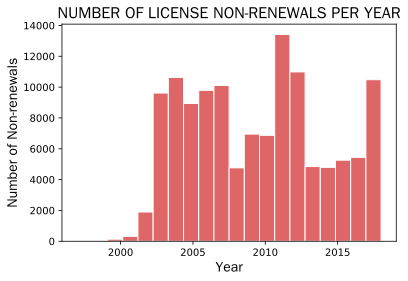
\includegraphics[scale=0.5]{../../explorations/non-renewals-over-time.png}\\
\centering{Figure 1: Number of failures per year}
\end{minipage}\hfill\begin{minipage}[t]{0.4\pagewidth}
\vspace{0pt}
\includegraphics[scale=0.5]{../../explorations/failure-choropleth.png}\\
\centering{Figure 2: Geographic distribution of business failures}
\end{minipage}
\begin{table}[H]
\centering \small \renewcommand{\arraystretch}{1.1}
\begin{tabular}{l|r}
\opns{business activity}                                                                    & \opns{\% of  failures} \\\hline
Operation of a Fuel Filling Station                                                  & 23.49                 \\
Retail Sales of Perishable Foods                                                     & 12.31                 \\
Buying and Reselling of Used Valuable Objects                                        & 10.47                 \\
Consumption of Liquor on Premises                                                    & 3.99                  \\
Mobile Desserts Vendor & 2.74                  \\
Tavern - Consumption of Liquor on Premise                                            & 1.87                  \\
Hair Services                                                                        & 1.67                  \\
Preparation of Food and Dining on Premise With Seating                               & 1.62                  \\
Other Home Occupations                                                               & 1.61                  \\
Miscellaneous Commercial Services                                                    & 1.42                 
\end{tabular}
\caption{Business types by propensity to fail}
\end{table}

The table below lists our proposed set of initial features and a description of each.
\begin{table}[H]
\centering \small \renewcommand{\arraystretch}{1.1}
\begin{tabular}{l|l}
\opns{Feature}                                     & \opns{Description} \\\hline
Year                                        & The time-granularity at which we can focus \\
Ward                                        & In which city ward the business is located                           \\
Number of prior license renewals            & The number of times the given license has been renewed               \\
Number of businesses owned by account owner & Account owners may own more than one business                        \\
Business activity                           & Type of business (retail, food sales, services, etc.)                \\
is national chain                           & If business is a franchise of national chain                         \\
received TIF                                & If business received Tax Incremental Financing                       \\
received SBIF grant                         & If business received a grant from the Small Business Innovation Fund \\
located in SSA                              & If business is located in a Chicago business improvement district    \\
National GDP in given year                  & Gross domestic product for the entire US                             \\
Illinois state GDP in given year            & Gross domestic product for the state of Illinois                     \\
Cook County GDP in given year               & Gross domestic product for Cook County                               \\
\textbf{Business active in given year}             & \textbf{Column to predict}
\end{tabular}
\caption{Description of machine learning model features}
\end{table}
\subsection{Machine learning approach}
Our goal is to generate a model that will predict whether a business is likely to still exist two years after having applied for or renewed its business license.  

We plan to test a variety of different machine learning methods using a range of parameters to identify which method and set of parameters seems to perform best on this problem. These methods include the following:
\begin{itemize}
\item Decision trees: Simple decision trees of depths one to three will help us understand which individual features seem to be most important in predicting whether a business survives. 
\item Logistic regression: The weights from such models can help us understand the relative importance of the different features we use to predict business survival.
\item Support vector machines (SVM): SVM models will allow us to explore whether a nonlinear decision boundary might perform better at predicting business survival.
\end{itemize}
In addition, we will employ ensemble methods, such as random forests, bootstrap aggregation, and gradient boosting, to improve the performance of these classifiers. 

\subsection{How will we evaluate our models?}
To choose between the models we develop using the methods described in the last section, we will pursue a temporal cross-validation strategy. For a given date $T_0$, we will train our models only on business licenses applications and renewals occurring prior to $T_0$. Subsequently, we evaluate model performance using the presence or absence of a business license renewal in the two years following $T_0$. We exclude businesses whose license terms do not expire within the two years following $T_0$, as we cannot reasonably assume that these businesses have either survived or failed. We will perform this evaluation using the sliding window method, in which our training set will be limited to the two years prior to $T_0$, as well as the expanding window method, in which our training set will include all data prior to $T_0$.

To evaluate model performance, we will compute precision (the share of true surviving businesses in our predicted survivors) and recall (the share of true survivors that we correctly predicted) using a range of thresholds to convert prediction scores into a binary classification. We will compare our models' performance on these metrics to a few simple baselines:
\begin{itemize}
\item Do our models have better precision/recall than random chance? For example, if $X$ percent of businesses fail within two years, our model should perform better than choosing $X$ percent at random. 
\item Do our models perform better than a simple majority classifier? 
\item Do they provide more insight or perform better than a very simple decision tree stump? This comparison could serve as a proxy for the heuristics used by existing organizations. 
\end{itemize}

After we deploy a model, we would want to continue assessing its performance over time to ensure that its predictions do not markedly decrease in quality. We could consider randomized interventions or other field tests to assess both the accuracy of our predictions and the effectiveness of any assistance extended to the businesses we identify as struggling. 

\subsection{Caveats and limitations}
Our analysis has a number of limitations, and should be considered in light of the following caveats:
\begin{itemize}
\item We do not observe any measures of individual business viability or performance, such as revenue, profits, number of employees, or production. This limits our ability to predict the success or failure of a business to the fundamentals of the business type, rather than the specific business model or performance of a specific business. Consequently, we will not be able to clearly distinguish businesses that are struggling but have viable business plans from those that lack such plans.
\item Not all businesses in Chicago are required to obtain business licenses from the city, and as a result, these businesses are not included in our dataset.\footnote{\url{https://www.chicago.gov/city/en/depts/bacp/sbc/business_licenseexemption.html}} In particular, certain professions that are licensed by state boards are exempt from municipal business requirements. Notable examples of such business types include accountants, cosmetology schools and similar businesses, and a wide range of healthcare practitioners. Given that these exempt businesses are likely to be unevenly distributed across the city and may cluster near non-exempt types of businesses, the lack of data on exempt businesses may bias our predictions about clusters of business failures. 
\item Our model does not treat certain types of businesses as “better” for overall community quality of life; it merely predicts business survival. Policymakers might reasonably decide not to assist certain types of businesses that we predict as likely to fail if they believe the business - for example, a liquor store or payday loan operation - would negatively impact neighborhood quality of life.
\end{itemize}

\subsection{Ethical issues, bias, and fairness}
Developing and deploying such a model to guide resource allocation decisions raises important ethical questions about bias and fairness. In particular, we are concerned about the following issues:
\begin{itemize}
\item Our data necessarily reflect historical patterns of (dis-)investment in particular Chicago neighborhoods that manifest themselves along racial lines. For this reason, our model may predict that businesses located in historically disadvantaged communities are less likely to succeed. Additionally, data may be less rich in such communities. Any decision about resource allocation made based on the predictions we generate must be cognizant of these historical patterns. 
\item Our model will generate failure risk scores and classify businesses as likely to fail or not based on these scores. Implicitly, this approach assumes that the businesses predicted to be most likely to fail would be targeted for intervention. If the fact that a business is selected for intervention becomes publicly known, it could negatively affect the business by branding it as “failing,” potentially harming the business instead of helping it. In other words, the general equilibrium effects of introducing this sort of predictive assistance are difficult to predict and could be counterproductive.
\item Our model could predict that the least-viable businesses are those at highest risk of failure. From the perspective of a decisionmaker tasked with allocating public or philanthropic dollars in the most effective manner, assisting such businesses that are not viable to begin with may not be the right approach.

\end{itemize}

\section{Recommendations for Policy}
\subsection{Summary of recommendations}
The predictions from our model(s) could be aggregated to determine neighborhoods with a high risk of concentrated business closure, potentially looking specifically at small businesses. Economic development agencies and city government officials could then prioritize those neighborhoods for preemptive outreach in terms of financial and technical business assistance. 

Other entities that rehabilitate economically depressed neighborhoods could use the predictions from our model to inform medium-term financial planning. If found to be sufficiently precise, our point estimates of risk of business failure could even be used to evaluate other business-related interventions. For example, the NHS, whose Micro Market Recovery Program (MMRP) seeks to revive such neighborhoods, could estimate changes in risk scores for businesses in their target markets as validation that their programs were achieving their goals.

